Le très fameux algorithme d'Euclide connu par les grecs anciens, est fortement lié aux fractions continues. Cependant nous avons aucun écrits sugérant que les grecs auraient utilisé cet algorithme pour calculer autre chose que des plus grands diviseurs communs.\newline

Les premières traces dans l'histoire de l'usage des fractions continues remontent à l'Inde ancienne. Aryabhata, un mathématicien et astronome du Vème siecle, s'en sert pour calculer des racines carrées.\newline

Puis dans la littérature arabe et européenne à l'époque médivale, elles réapparaissent plusieurs fois mais toujours pour calculer des cas particuliers.\newline

Dans le livre Opera Mathematica en 1965 le mathématicien Wallis pose les bases de la théorie des fractions continues. Il explique comment calculer le nième terme et découvre certaine propriétés.\newline

L'astronome Huygens cherchant à créer un automate imitant le système planétaire les utiliseras pour trouver une approximation fractionelle du ratio entre la durée d'une année terrestre et une année de Saturne.\newline
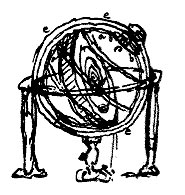
\includegraphics[width=6cm]{Image/Automate_planetaire_de_Huygens.jpg}
En 1737 Leonhard Euler écrit De Fractionlous Continious où il dévellope la théorie moderne des fractions continues. Son principal résultat est d'arrive à calculer le dévellopement en fraction continue de la constante $e$. \[
e=[2,1,2,1,1,4,1,1,8,1,...,1,2k,1,...]
\]
Ce dévellopement est infini ce qui prouve que $e$ est un irrationel. C'est la première démonstration de ce résultat.\newline

Elles seront également utilisées pour des travaux sur les nombres transcendant. Liouville en utilise une pour exhiber le premier nombre transcendant. Puis Charles Hermite démontre la transcendance de $e$ en 1873 et Ferdinand von Lindemann celle de $\pi$ grace à une méthode metant en oeuvre des fractions continues. \newline%TODO trouver les articles

Ces méthodes s'étant relevée efficace, la communauté mathématique a voulu l'élargir a des dimensions supérieurs. Ainsi pour calculer des suite de fraction s'approchant d'un vecteur donné, plusieurs méthodes ont vu le jour. Cependant contrement au cas de la dimension un, il n'y a pas unicité de la façon de faire. La diversité des algorithme en résultant a donc apporter aussi un lot ede question. Il faut comprendre lequel converge et quantifier la vitesse de convergence.

L'apport de la théorie dynamique a apportée un regard plus analystique et topologique a cette question qui relevait d'habitude plus de la théorie des nombres. C'est donc ainsi que mon stage a consister à analyser la preuve de la convergence forte d'un algorithme et à essayer de l'adapter à d'autres.
